\documentclass[11pt]{article}
\usepackage[margin=1in]{geometry}
\usepackage[T1]{fontenc}
\usepackage[sc]{mathpazo}
\linespread{1.05}
\usepackage{microtype}
\usepackage{amsmath,amssymb,amsthm,mathtools}
\usepackage{booktabs}
\usepackage{longtable}
\usepackage{graphicx}
\graphicspath{{./}}
\usepackage{float}
\usepackage{enumitem}
\usepackage{xcolor}
\usepackage{tikz}
\usetikzlibrary{arrows.meta,calc}
\usepackage[hidelinks]{hyperref}
\usepackage[capitalise,noabbrev]{cleveref}
\newtheorem{theorem}{Theorem}[section]
\newtheorem{lemma}[theorem]{Lemma}
\newtheorem{proposition}[theorem]{Proposition}
\newtheorem{corollary}[theorem]{Corollary}
\theoremstyle{definition}
\newtheorem{definition}[theorem]{Definition}
\newtheorem{designrule}[theorem]{Design rule}
\theoremstyle{remark}
\newtheorem{remark}[theorem]{Remark}
\crefname{designrule}{Design rule}{Design rules}
\newcommand{\norm}[1]{\lVert #1 \rVert}
\newcommand{\AU}{\,\mathrm{AU}}
\newcommand{\h}{\,\mathrm{h}}
\newcommand{\km}{\,\mathrm{km}}
\newcommand{\vmax}{v_{\max}}
\newcommand{\lfl}{\ell^{\mathrm{floor}}}
\title{The MultiPlanetary Exchange:\\ A Light-Speed Market Design with Proven Connectivity}
\author{Jose Cisneros and Benjamin Robertson\\ \small Gator Quant Hacks 2026, Quantitative Puzzles track}
\date{October 2026}
\begin{document}
\maketitle
\begin{abstract}
MPX clears trades for nine settlements at an Earth hub over the brief's relay backbone. Mercury through Jupiter clear every 90 minutes; Saturn, Uranus and Neptune join every fourth batch. Deadlines use the straight-line light-time, so no accepted order can use information from after its cutoff on any path. Deadline messages travel as independent copies sized from the exactly predictable loss, reaching $99.5\%$ on-time in every geometry of 200 years within the 600-origination quota. Transfers are exactly once by construction: only the destination can declare a transfer credited or never credited. Margin covers fat-tailed prices over each member's worst round trip, members hold liquidity of $30\%$ of notional, and a Cover-2 fund is prefunded at the hub. Every number is reproducible from the shipped scripts; all eight toolkit checks pass.
\end{abstract}
\vspace{-4pt}
\noindent\fbox{\parbox{\dimexpr\linewidth-2\fboxsep-2\fboxrule}{\small\textbf{Contributions.}
(1) A proof that the Sun can never cut the backbone, and a 200-year scan that provably misses no closure.
(2) \emph{Light-Cone Clearing}: batch deadlines set by straight-line light-time, fair on every path, including the faster direct service.
(3) Exactly-once transfers, atomic cross-planet swaps and a single active hub, each with a proof.
(4) Order copies sized from exactly predictable loss: $99.5\%$ on time in every geometry of 200 years within the 600-origination quota.
(5) A mapped failure boundary: the member liquidity at which defaults begin, for rising and falling prices alike.}}
\vspace{2pt}

In 1974 Bankhaus Herstatt failed after receiving one leg of its currency trades and before paying the other, because the second leg was due hours later in another time zone \cite{bisfx}. MPX faces the same problem with light-hours instead of time zones, and resolves it the same way: no obligation is settled on one side before it can be settled on the other.
\vspace{-6pt}
\section{Architecture}\label{sec:arch}
\textbf{Actors.} The \emph{hub} at Earth runs matching and the clearing ledger (members' margin, default fund, MPX capital). Each settlement runs a \emph{home ledger}, the only writer of its clients' cash accounts. \emph{Members} clear at the hub: banks inside Saturn's orbit, and one \emph{operator} per settlement beyond Saturn, which clears for its local clients. Relays A and B forward packets. All messages are signed and carry a unique ID (origin, sequence).

All rules of the model are the brief's \cite{brief}. \textbf{Network facts we rely on} (proved in \cref{sec:guar}, measured in E4): the A--B link never closes; the Sun never blocks both relays from one settlement; every settlement pair has an open route of at most three links at every hour of 200 years.
\begin{figure}[H]
\centering
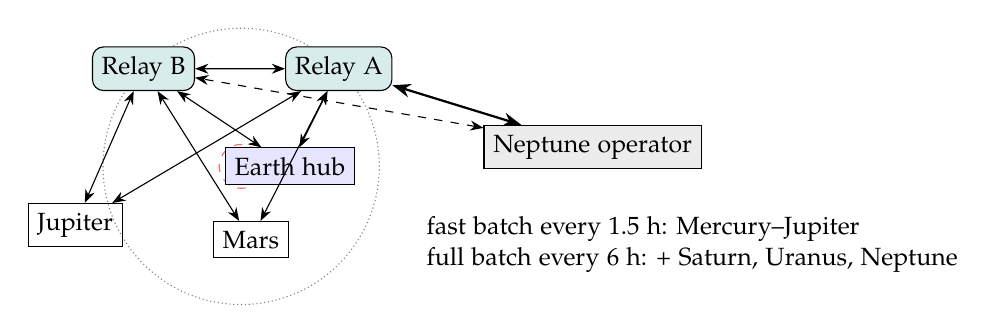
\begin{tikzpicture}[scale=0.62,>=Stealth,font=\small]
\fill[orange!70] (0,0) circle (0.18); \draw[red!60,dashed] (0,0) circle (0.45);
\draw[gray,densely dotted] (0,0) circle (2.83);
\node[draw,fill=teal!15,rounded corners] (A) at (2,2) {Relay A}; \node[draw,fill=teal!15,rounded corners] (B) at (-2,2) {Relay B};
\node[draw,fill=blue!10] (E) at (1.0,0) {Earth hub};
\node[draw] (M) at (0.2,-1.5) {Mars}; \node[draw] (J) at (-3.4,-1.2) {Jupiter};
\node[draw,fill=gray!15] (N) at (7.2,0.4) {Neptune operator};
\draw[<->] (A)--(B); \draw[<->] (E)--(A); \draw[<->] (E)--(B); \draw[<->] (M)--(A); \draw[<->] (M)--(B); \draw[<->] (J)--(B); \draw[<->] (J)--(A);
\draw[<->,thick] (N)--(A); \draw[<->,dashed] (N)--(B);
\node[align=left,anchor=west] at (3.6,-1.6) {fast batch every 1.5 h: Mercury--Jupiter\\ full batch every 6 h: + Saturn, Uranus, Neptune};
\end{tikzpicture}
\caption{Topology (not to scale). Every settlement links to both relays; A--B links the relays.}
\end{figure}
\vspace{-8pt}
\section{Operating rulebook}\label{sec:rules}
\textbf{R1 Sessions.} Each settlement pins the earliest-arriving open candidate route and re-pins, by a one-origination handshake, before every closure predicted from the frozen elements. If all candidates are closed (maintenance, incident), packets hold at the last open node.

\textbf{R2 Batches.} A fast batch clears every $B=1.5\h$ for settlements whose straight-line light-time to Earth never exceeds $0.9\h$ (Mercury, Venus, Earth, Mars, Ceres, Jupiter). Every fourth batch is a full batch that also admits Saturn, Uranus and Neptune. Settlement $k$'s order for cutoff $T_b$ is valid only if it arrives by $D_k = T_b + \lfl(k\to\text{Earth},T_b)$. Settlement $k$ sends at $T_b - (\ell_k - \lfl_k) - 60\,$s, its route's excess over the straight line plus a one-minute margin. The batch clears at $T_b+\max\lfl$ over admitted settlements, fills at one uniform price as in frequent batch auctions \cite{budish2015}, and broadcasts the list of accepted order IDs. The outer cadence is forced by the quota: admitting Saturn, Uranus and Neptune every 3 hours would leave 48 originations of reserve on the worst day of 200 years, below the 56 that margin calls alone reached in E5; every 6 hours leaves 132.

\textbf{R3 Copies and deduplication.} A deadline message is sent as $k$ independent originations, with $k=\lceil\ln 0.005/\ln(1-f)\rceil$ for the route's first-try success $f$, which geometry determines exactly in advance. The receiver acts on the first valid copy of an ID and receipts but ignores the rest. Non-deadline messages (results, statements) go once and rely on hop retries.

\textbf{R4 Late and missing orders.} An order arriving after $D_k$ is \emph{rejected late}, never rolled forward; the accepted-ID broadcast tells the sender, who may resubmit for the next batch.

\textbf{R5 Transfers.} The source ledger debits the amount into a \emph{hold} and sends TRANSFER with expiry $E = t_0 + \min(30\text{ days},\,4R_e)$, four endpoint-retry intervals, which is $100$--$129\h$ depending on the settlement. The destination credits the first copy that arrives before $E$ and returns CREDITED. After $E$, or earlier on the source's CANCEL request, a destination that never credited the ID \emph{tombstones} it, rejects every later copy, and signs NOT-CREDITED; a refund therefore takes one round trip, not 30 days. The source finalizes on CREDITED and refunds on NOT-CREDITED, \emph{never} on a timeout. Funds in flight earn no interest.

\begin{figure}[H]
\centering
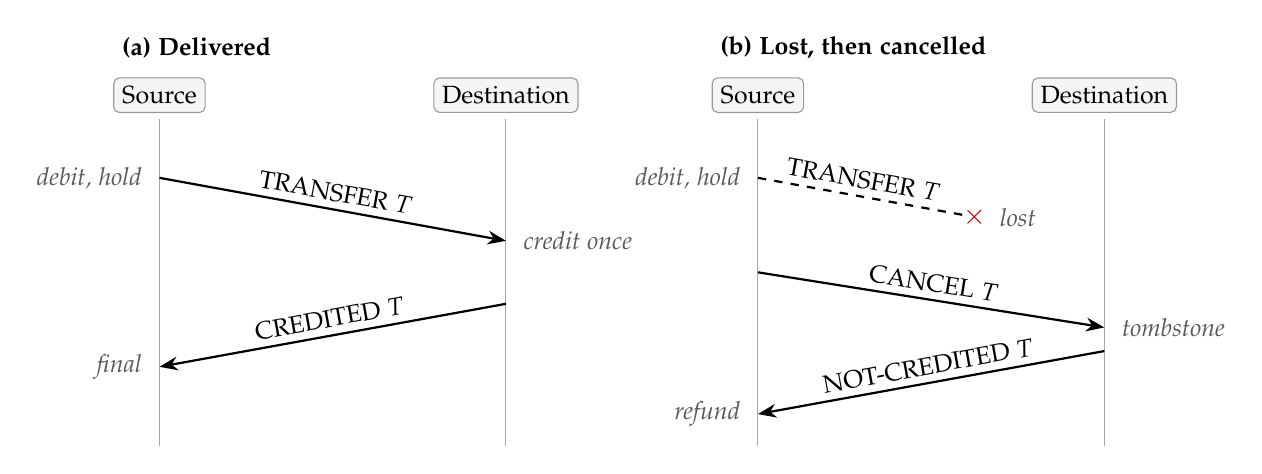
\begin{tikzpicture}[>=Stealth,font=\small,
  lbl/.style={midway,above=1pt,sloped,fill=white,inner sep=1.5pt},
  note/.style={font=\small\itshape,text=black!65},
  head/.style={draw=black!40,rounded corners=2pt,fill=black!4,inner sep=3pt,font=\small}]
\node[font=\small\bfseries,anchor=west] at (-0.6,0.95) {(a) Delivered};
\node[head] at (0,0.35) {Source}; \node[head] at (4.4,0.35) {Destination};
\draw[black!35] (0,0.05)--(0,-4.1); \draw[black!35] (4.4,0.05)--(4.4,-4.1);
\draw[->,thick] (0,-0.7)--node[lbl]{TRANSFER $T$}(4.4,-1.5);
\node[note,anchor=east] at (-0.1,-0.7) {debit, hold};
\node[note,anchor=west] at (4.5,-1.5) {credit once};
\draw[->,thick] (4.4,-2.3)--node[lbl]{CREDITED $T$}(0,-3.1);
\node[note,anchor=east] at (-0.1,-3.1) {final};
\begin{scope}[xshift=7.6cm]
\node[font=\small\bfseries,anchor=west] at (-0.6,0.95) {(b) Lost, then cancelled};
\node[head] at (0,0.35) {Source}; \node[head] at (4.4,0.35) {Destination};
\draw[black!35] (0,0.05)--(0,-4.1); \draw[black!35] (4.4,0.05)--(4.4,-4.1);
\draw[thick,dashed] (0,-0.7)--node[lbl]{TRANSFER $T$}(2.6,-1.17);
\node[text=red!70!black,font=\bfseries] at (2.75,-1.2) {$\times$};
\node[note,anchor=west] at (2.95,-1.2) {lost};
\node[note,anchor=east] at (-0.1,-0.7) {debit, hold};
\draw[->,thick] (0,-1.9)--node[lbl]{CANCEL $T$}(4.4,-2.6);
\node[note,anchor=west] at (4.5,-2.6) {tombstone};
\draw[->,thick] (4.4,-2.9)--node[lbl]{NOT-CREDITED $T$}(0,-3.7);
\node[note,anchor=east] at (-0.1,-3.7) {refund};
\end{scope}
\end{tikzpicture}
\caption{R5 transfers. (a) The destination credits the first copy and signs CREDITED. (b) A lost transfer is cancelled; the destination's signed decision, never a timeout, releases the source's hold.}
\end{figure}
\vspace{-4pt}
\textbf{R6 Margin.} All collateral sits at the hub. Initial margin is $\mathrm{IM}=2.62\,\sigma\sqrt{\mathrm{MPOR}}\,N$, with $\mathrm{MPOR}=$ worst 200-year round trip $+\,G+B$, $G=1\h$. Variation margin settles inside the hub at every batch. If collateral falls below $80\%$ of IM, the hub sends a call (as copies) to restore IM, due one round trip plus $G$ later. An unanswered call is resent once; a member defaults only if the resent call also goes unanswered, or if it cannot pay. Members must hold liquid resources of $30\%$ of notional.

\textbf{R7 Default.} The hub closes out the position within one fast batch among members whose round trip is under $1.5\h$, then applies the waterfall: the defaulter's margin, unpaid variation margin and fund share; MPX capital ($25\%$ of the fund); survivors' shares; assessments of up to $1\times$ shares (prefunded in hub escrow beyond Saturn); then haircut variation-margin gains and partial tear-up. The fund is Cover 2 \cite{pfmi} at a $6\,$sd shock: $F=\max_{i\ne j}(S_i+S_j)$, $S_i=(6-2.62)\sigma\sqrt{\mathrm{MPOR}_i}N_i$.

\textbf{R8b Cross-planet swaps.} Assets held at the hub settle payment-versus-payment on the hub's books, both legs at once. An asset held on a home ledger is swapped by hash lock: the buyer locks credits under hash $H$, the seller locks the asset under $H$, the buyer claims the asset by revealing the secret, and the seller claims the credits with it. The seller's lock must outlast the buyer's claim plus one hour; the buyer's lock must outlast the seller's lock by one more light-time plus one hour.

\textbf{R8c Operator local markets.} An operator may run a continuous local market for its clients, quoting within $\text{hub price}\pm(2.62\,\sigma\sqrt{\ell}+0.10\%)$, where $\ell$ is the current light-time from the hub. It nets client flow into one order per full batch.

\textbf{R8d Netting and receipts.} Transfers between the same two ledgers are netted each batch, and relays acknowledge all copies of a batch with one aggregate receipt per hop, as in delay-tolerant networking.

\textbf{R8e Quota priority.} When less than the 132-origination reserve remains in the rolling 24 hours, originations go in this order: margin calls and their answers, incident notices and re-pins, orders, transfers, then statements, which are deferred and merged into the next result.

\textbf{R8f Hub continuity.} A standby hub at Mars mirrors every batch. Earth clears only while it holds a 4-hour lease that Mars has acknowledged; renewals and acknowledgments ride on the batch messages already exchanged with Mars, so they cost no extra originations. Mars may start clearing only after 5 hours without a renewal, after Earth's lease has expired, so the two never clear at once.

\textbf{R8 Incidents.} An incident notice goes out by the direct service and by the backbone. Sessions through an affected relay re-pin at once. A member isolated longer than its MPOR is \emph{hedged, not defaulted}: the hub closes its hub position into a hedge funded by its own margin and returns it at the hedge price when contact resumes.
\section{Products and service table}\label{sec:service}
MPX offers four products: \emph{transfers} between home ledgers; \emph{spot} in lots of $1{,}000$ units, tick $0.01$ credits; \emph{futures} with TDB expiries, cash-settled at the expiry batch price; and a \emph{delivery guarantee} paying face value if a transfer's endpoint attempt is abandoned, at a fair premium equal to that probability. Spot and futures require margin (R6) and member liquidity of $30\%$ of notional. Clearing fees, the operators' $0.10\%$ band fee and the guarantee loading fund MPX's operating capital.
\begin{table}[H]
\centering
\caption{Service at hour 0 by settlement ($\sigma=30\%$). Transfer times are to the Earth hub: credit after one way, final after the confirmation returns.}\label{tab:service}
\small
\begin{tabular}{@{}lp{0.13\linewidth}lp{0.1\linewidth}lp{0.11\linewidth}p{0.2\linewidth}@{}}
\toprule
Settlement & Access, batch & Copies & Credit / final (h) & Margin & Guarantee premium & Restrictions \\
\midrule
Mercury & member, fast & 3--4 & 0.77 / 1.53 & 1.93\% & $2.0\times10^{-5}$ & send up to 76 min early \\
Venus & member, fast & 3--4 & 0.68 / 1.35 & 1.94\% & $1.1\times10^{-5}$ & \\
Earth & hub, fast & 1 & local & 1.33\% & 0 & \\
Mars & member, fast & 2--4 & 0.57 / 1.13 & 1.95\% & $5.4\times10^{-6}$ & \\
Ceres & member, fast & 2--4 & 0.56 / 1.11 & 1.98\% & $5.2\times10^{-6}$ & B link closed h 240--264 \\
Jupiter & member, fast & 3--4 & 0.85 / 1.70 & 2.09\% & $2.9\times10^{-5}$ & \\
Saturn & member, full & 3--5 & 1.32 / 2.65 & 2.27\% & $3.4\times10^{-4}$ & orders every 6 h only \\
Uranus & operator, full + local & 5--7 & 2.64 / 5.28 & 2.67\% & $6.6\times10^{-3}$ & local quotes within $\pm1.46\%$ \\
Neptune & operator, full + local & 7--9 & 4.17 / 8.35 & 3.01\% & $3.3\times10^{-2}$ & local quotes within $\pm1.82\%$; B closed h 2--26 \\
\bottomrule
\end{tabular}
\end{table}
\vspace{-6pt}
\section{Responsibilities when messages fail}\label{sec:fail}
Authority is fixed: the hub decides batches, fills and margin; the destination ledger decides whether a transfer was credited; the source ledger decides debits. No actor ever infers another's decision from silence.
\begin{table}[H]
\centering
\caption{What each actor knows, does and owes.}\label{tab:fail}
\small
\begin{tabular}{@{}p{0.13\linewidth}p{0.26\linewidth}p{0.26\linewidth}p{0.26\linewidth}@{}}
\toprule
Failure & Order (sender, hub) & Transfer (source, destination) & Margin call (hub, member) \\
\midrule
Lost & Hub knows nothing. Sender learns from the accepted-ID broadcast, owes nothing, may resubmit next batch & Hop retries, then endpoint attempts. Source knows only ``pending'', keeps the hold. Destination owes nothing until a copy arrives & Hub knows the call is unanswered at its deadline and resends once. Member owes the top-up from when it receives the call \\
Late & Rejected late (R4); listed as rejected. Sender's position unchanged & Valid until $E$ unless cancelled. After $E$ or a CANCEL, the destination tombstones it and signs NOT-CREDITED; the source refunds & A payment after the deadline still counts; default only after the resend round expires \\
Duplicated & First valid copy filled; others receipted and ignored. At most one fill per ID & First copy credited; later copies receipted, never credited twice & Repeat calls with the same ID ask for the same top-up once \\
Contradicted & Same ID, different content: both rejected, sender flagged; hub's record of fills is final & Destination's signed CREDITED or NOT-CREDITED is final; it can sign only one & Hub's statement prevails; disputes settle at the next batch statement \\
\bottomrule
\end{tabular}
\end{table}
\vspace{-6pt}
\begin{table}[H]
\centering
\caption{Order lifecycle. Each state has exactly one authority; no state is inferred from silence.}\label{tab:life}
\small
\begin{tabular}{@{}lp{0.12\linewidth}p{0.33\linewidth}p{0.3\linewidth}@{}}
\toprule
State & Authority & Entered when & Leaves to \\
\midrule
Created & sender & client submits; ID assigned & Sent \\
Sent & sender & $k$ copies launched by $T_b-(\ell-\lfl)-60\,$s & Valid or Rejected late \\
Valid & hub & first copy arrives by $D_k$ & Cleared \\
Rejected late & hub & no copy by $D_k$; listed in the accepted-ID broadcast & terminal; may resubmit \\
Cleared & hub & batch clears at $T_b+\max\lfl$ & Filled or Unfilled \\
Filled / Unfilled & hub & uniform-price match decided & Reported \\
Reported & hub & fill report sent; position and margin updated at the hub & Confirmed \\
Confirmed & sender & report received; sender's view matches the hub & terminal \\
\bottomrule
\end{tabular}
\end{table}
\vspace{-6pt}
\section{Assumptions}\label{sec:assume}
\begin{table}[H]
\centering
\caption{Assumptions, kept apart from proofs and limits.}\label{tab:assume}
\small
\begin{tabular}{@{}lp{0.56\linewidth}p{0.3\linewidth}@{}}
\toprule
\# & Assumption & Used by \\
\midrule
A1 & The brief's frozen ellipses, constants, loss model, quotas and maintenance are exact & everything \\
A2 & Launches are lost independently, as the brief states & copies, E2 \\
A3 & Price returns: $\sigma=30\%$ a year; Student-$t_3$ tails for margin & R6, E5 \\
A4 & Messages are signed; keys identify the origin settlement & G3, G4 \\
A5 & Members hold liquid resources of $30\%$ of notional, recertified monthly & R6, E5 \\
A6 & Batch, transfer and statement messages fit one packet each & quota counts \\
A7 & Deterministic S1 price paths of $\pm0.5\%$ per fast batch; the S2 incident is our choice & S1, S2 \\
A8 & Direct service is used only for incident notices, within its 12-copy daily allowance & E2 \\
\bottomrule
\end{tabular}
\end{table}
\vspace{-6pt}
\section{Guarantees and their conditions}\label{sec:guar}
\textbf{G1 Connectivity} (Sun only). Relays A and B share a $\sqrt8\AU$ circle, $90^\circ$ apart, so their chord passes the Sun at $2\AU$. For a settlement at radius $r$, a blocked relay lies within $\arcsin(0.1(1/r+1/\sqrt8))\le21.13^\circ$ of its antipode (worst case: Mercury at perihelion), so the two relays are never blocked together. \emph{Proof.} A closure needs the segment's nearest point to the Sun inside it (both endpoints lie at least $0.3075\AU$ out). Then the angle $\theta$ at the Sun between the settlement $P$ and the relay $R$ satisfies $\sin(\pi-\theta)\cdot r\sqrt8 = 2\cdot\text{area} = |P-R|\cdot\text{dist} \le |P-R|\,0.1 \le (r+\sqrt8)\,0.1$, giving the bound. The relays are $90^\circ$ apart and each blocked cone is at most $2\times21.13^\circ$ wide, so no direction blocks both. Projecting to the ecliptic only shortens distances, so the planar case covers 3D. $\square$ \emph{Condition:} no maintenance or incident on both a settlement's relay links.

\textbf{G2 No closure missed.} Clearance is $V$-Lipschitz with $V=\max(v_s, v_r(1+2\vmax/(c-\vmax)))$ (perihelion speeds), so an hourly sample below $0.10+V/2$ flags every closure; flagged hours are refined to 1 minute and boundaries bisected to $10^{-7}\h$.

\begin{figure}[H]
\centering
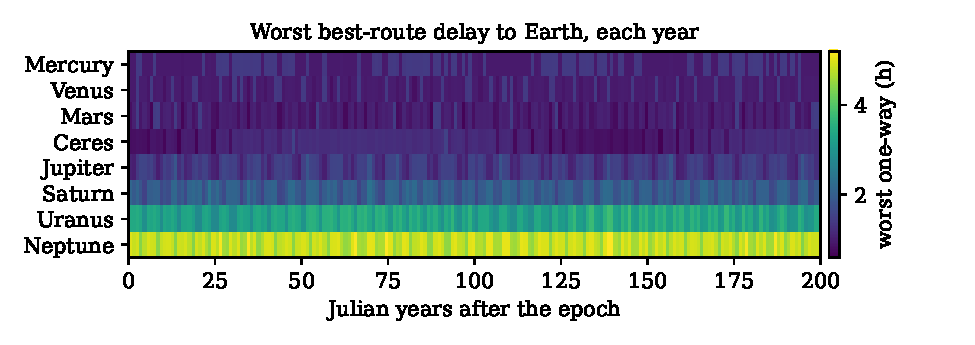
\includegraphics[width=\linewidth]{fig_heatmap.pdf}
\vspace{-14pt}
\caption{E4 at a glance: the worst best-route delay to Earth in each of 200 years. Every cell is finite (G1); Neptune never exceeds $5.19\h$.}
\end{figure}
\vspace{-6pt}
\textbf{G3 Causal fairness (Light-Cone Clearing).} An order arriving by $T_b+\lfl$ left its origin by $T_b$, since no path beats the straight line, including the faster direct service. \emph{Condition:} the hub knows each order's origin (signed keys).

\textbf{G4 Exactly-once transfers and conservation.} The destination signs at most one of CREDITED or NOT-CREDITED per ID: it credits only an ID it has not tombstoned, and it tombstones (signing NOT-CREDITED) only an ID it has not credited; both decisions are local to one single-writer ledger, so they cannot both occur. The source moves the hold exactly once, on that signature. At every instant each unit of value is in exactly one place: available, held at the source, in flight, or credited at the destination. Total funding is constant, and no unit is spendable in two places. \emph{Proof.} Every ledger action is a double entry summing to zero, so total funding is invariant. Transfer $T$ has three phases: before credit (value in flight, source holds a non-spendable memo), credited (spendable only at the destination), refunded (spendable only at the source). Credit and tombstone are mutually exclusive decisions of one single-writer ledger. The source moves only on the destination's signed decision. Hence $T$ ends credited or refunded, never both, and no phase makes the value spendable in two places. Retries and copies carry the same ID, so they can trigger at most one credit. $\square$ (E3 checks this in every scenario.)

\textbf{G5 At most one fill per order}, by ID deduplication (R3); copies can never multiply a position.

\textbf{G6 On-time deadline messages}: probability at least $99.5\%$, from $f$ at send time. \emph{Condition:} independent launches, which incidents break (handled by R8, not by probability).

\textbf{G7 Margin coverage.} IM covers $99\%$ of price moves over the MPOR for Student-$t_3$ returns; Gaussian returns exceed it only $0.45\%$ of the time (E5). \emph{Condition:} the call is delivered. A call or answer misses its first window with probability at most $1-0.995^2=1.0\%$; the resend then stretches Neptune's window from $12.9$ to $23.3\h$, where $t_3$ exceedance is $2.16\%$. The total is $0.99\times1.0016\%+0.01\times2.16\%=1.013\%$.

\textbf{G9 Swap atomicity.} A hash-locked swap ends with both legs done or both refunded. \emph{Proof.} The seller can claim only with the secret, which the buyer reveals only by claiming the asset; once revealed, the secret reaches the buyer's ledger within one light-time, and the buyer's lock outlasts that. If the buyer never claims, both locks expire and each side refunds. $\square$ \emph{Condition:} locks set as in R8b.

\textbf{G10 One hub at a time.} If Mars last received a renewal sent at time $r$, Earth's lease ended by $r+4\h$, while Mars waits until at least $r+5\h$. Earth counts only renewals Mars has acknowledged, so its view is never later than Mars's. Their clearing intervals cannot overlap. $\square$ \emph{Condition:} both hubs keep TDB time (R1 clocks).

\textbf{G8 Finality bound.} No ledger can confirm a spend faster than light can reach another replica that could approve a conflicting one; single-writer home ledgers satisfy this by design \cite{gilbert2002}.

\section{Risks and limits}\label{sec:risk}
\begin{table}[H]
\centering
\caption{Ranked risks: severity and likelihood from 1 to 3, rank by their product, ties broken by severity.}\label{tab:risk}
\small
\begin{tabular}{@{}rp{0.18\linewidth}ccp{0.27\linewidth}p{0.27\linewidth}@{}}
\toprule
\# & Risk & Sev & Lik & Evidence & Control \\
\midrule
1 & Trend exhausts member liquidity & 3 & 2 & 15\% trend, 10\% jump and isolation: $18.45\%$ of rising runs default (E5) & 30\% liquidity rule; Cover-2 fund at 6\,sd; recovery used in 0.03--0.05\% of runs \\
2 & Outer member isolated (incident on top of maintenance) & 3 & 2 & Relay A loss h 0--6 with B--Neptune maintenance isolates Neptune (S2) & Notice by direct service; re-pin; hedge, not default (R8) \\
3 & Queue overflow on a pinned route & 3 & 1 & Cap fills in $16.7$ days; closures last up to $190$ days & Re-pin before every predicted closure (R1) \\
4 & Lost margin call & 2 & 2 & $0.2$--$0.4\%$ of calls miss on first send (E5) & Copies; one resend round before default (R6) \\
5 & Fat-tailed prices & 2 & 2 & Gaussian multiplier breached $1.38\%$ (E5) & Multiplier 2.62; 6\,sd fund stress \\
6 & Quota crunch on incident days & 2 & 1 & Worst day 468 for batches; calls peak at 56 a day & 132 originations reserved; adaptive copies \\
7 & Model error vs real ephemeris & 1 & 3 & Earth drifts up to about 4{,}700 km, $15.6$\,ms (\cref{sec:effects}) & 60 s send-early margin \\
8 & Duplicates and conflicts & 3 & 1 & Copies, retries and receipts all create duplicates & ID deduplication; authority table (\cref{tab:fail}) \\
9 & Hub outage at Earth & 3 & 1 & Earth is a single clearing point & Mars standby with leases; no overlap (R8f, G10) \\
10 & Quota exhausted mid-incident & 2 & 1 & Calls, re-pins and orders compete & Fixed priority order (R8e) \\
\bottomrule
\end{tabular}
\end{table}
\begin{figure}[H]
\centering
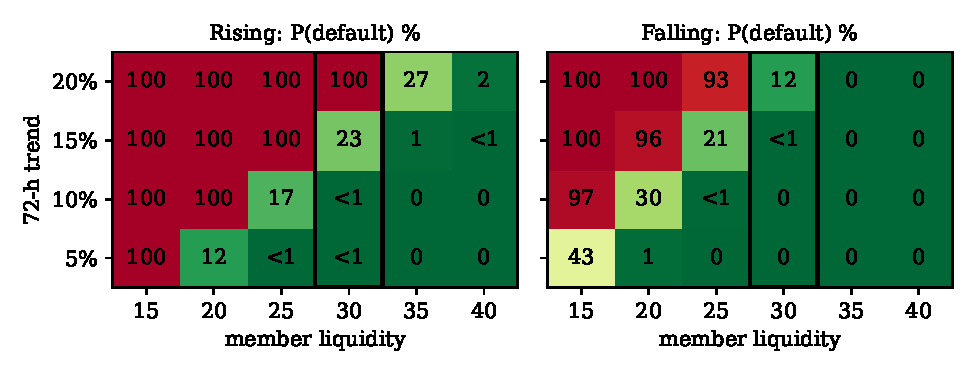
\includegraphics[width=\linewidth]{fig_phase.pdf}
\vspace{-14pt}
\caption{Failure boundary (E5 Tier 3, 600 runs per cell): probability of a member default against member liquidity and the 72-hour trend, with a 10\% jump, fat tails and a Neptune isolation on top. The boxed column is the design's 30\% rule; defaults appear only when the trend outruns liquidity, in either direction.}
\end{figure}
\vspace{-6pt}
\textbf{Interactions.} (i) More copies raise on-time delivery but spend quota: adaptive copies cut the worst day from 496 to 468 originations. (ii) Straight-line deadlines make batches fair but cost Mercury up to 76 minutes of information. (iii) An isolation plus a falling price stresses margin while calls cannot be delivered: R8 caps exposure at the MPOR. (iv) Maintenance turns a 6-hour relay incident into a full Neptune isolation that would otherwise cost 45 minutes (S2). (v) The liquidity rule protects the waterfall but ties up $30\%$ of notional: capital efficiency trades against default risk (E5 sensitivity).

\textbf{Limits.} Batches clear at most every $1.5\h$; Saturn, Uranus and Neptune trade every $6\h$; positions need liquidity of $30\%$ of notional; a refund needs the destination's signature, one round trip after CANCEL (up to $10.4\h$ for Neptune).
\section{Economic performance}\label{sec:econ}
\begin{table}[H]
\centering
\caption{Performance at hour 0 (S1, S3) and over 200 years (E4, quota scan).}\label{tab:econ}
\small
\begin{tabular}{@{}p{0.3\linewidth}p{0.62\linewidth}@{}}
\toprule
Measure & Result \\
\midrule
Access & Every settlement has an open route at every hour of 200 years; 24-hour availability $1.000$ at hours 0 and 300. Outer clients trade continuously on their operator's local market, whose quotes stayed inside the band in both price runs \\
Completion: transfer to hub & Credit $0.56\h$ (Ceres), $0.85\h$ (Jupiter, median), $4.17\h$ (Neptune); final after $1.11$, $1.70$, $8.35\h$ \\
Completion: order to fill & Inner: cutoff wait $\le1.5\h$, clearing lag $\le0.89\h$. Outer: cutoff wait $\le6\h$, clearing lag $\le4.35\h$ \\
Completion: price runs & Rising $15.2\h$, falling $26.0\h$ from first move until every top-up is final \\
Communication & 398 originations a day on average, 468 on the worst day of 200 years, of 600; worst link load $5.6\%$ of capacity \\
Capital & Initial margin $1.33$--$3.01\%$ of notional; prefunded resources $57.40$ for $1{,}500$ gross notional ($3.8\%$, breakdown in E3), against $4.6\%$ for a single three-hour batch \\
Recovery & S2: service restored within the incident plus one round trip; no obligation lost; collateral never negative \\
\bottomrule
\end{tabular}
\end{table}

\begin{figure}[H]
\centering
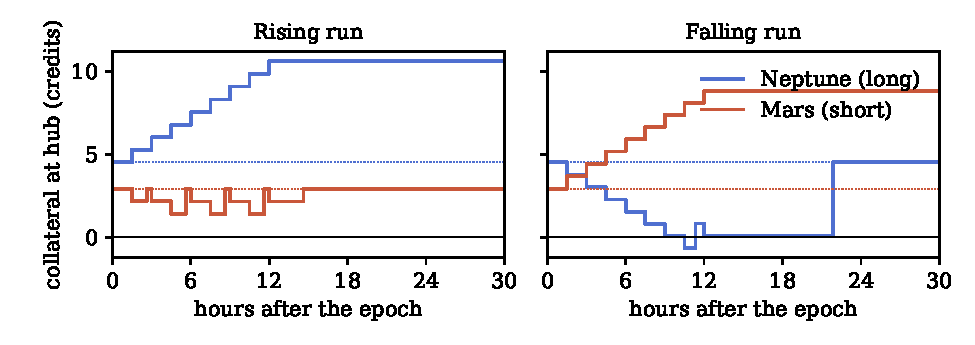
\includegraphics[width=\linewidth]{fig_runs.pdf}
\vspace{-14pt}
\caption{S1 price runs, weighted equally: collateral at the hub (solid) against initial margin (dotted). The losing side receives calls and tops up; Neptune's top-ups take a round trip of about 8 hours, yet its collateral never goes negative.}
\end{figure}
\vspace{-6pt}
\section{Continuing operation}\label{sec:cont}
MPX runs indefinitely on the frozen elements. Every closure in the next 200 years is known, so R1 schedules re-pins in advance: about $7.9$ a year for Mercury, $2.8$ for Venus, $1.6$ for Earth and fewer than one for the rest, at one origination each. Copy counts are recomputed for every send from the predicted geometry. The quota is budgeted on a rolling 24-hour window, with 132 originations held in reserve on the worst day. The fund is recalibrated with each book change, members recertify liquidity monthly, and timestamps are TDB throughout. The scenarios rerun at $+1$, $+10$ and $+100$ years and at the worst epoch of the 200-year scan with balances reset; completion times stay within $4.0\h$ of hour 0 and funding is conserved in every run (E5).

\section{Deployment assessment}\label{sec:deploy}
\textbf{What exists.} Every rule in this paper runs on the brief's frozen model: propagation, the 200-year closure scan, routing, loss and delivery, the protocol engine with its ledgers, and the stress runs. Two independent implementations agree to the last reported digit, and the toolkit's eight checks pass.

\textbf{What deployment needs.} A clearing service at Earth (matching, the clearing ledger, the fund); a home ledger at each settlement; operators at Uranus and Neptune with their escrow prefunded at the hub; relay software that sends one aggregate receipt per hop per batch; signing keys registered for every settlement; atomic clocks keeping TDB; and the Mars standby with leases (R8f).

\textbf{Order of rollout.} (1) Earth hub and the fast tier, Mercury to Jupiter, with transfers and spot. (2) Saturn and the full batch. (3) Operators at Uranus and Neptune, with their local markets and escrow. (4) Futures and cross-planet swaps. (5) The Mars standby. (6) The delivery guarantee, once observed loss confirms the model's abandonment rates. Each step adds load the quota analysis already covers.

\textbf{Acceptance tests.} Each deadline message on time with probability at least $99.5\%$; at most 468 originations on any day; daily reconciliation showing zero difference in total funding across all ledgers; margin exceeded in at most $1\%$ of margin periods, checked monthly.

\textbf{Known gaps.} The brief refers to a reference propagator that the v1.3 archive does not contain; ours reproduces the epoch table to $4.7\times10^{-7}\AU$ and we report the gap to the organizers. Fixed ellipses drift from the real ephemeris by up to about $16$\,ms of light-time (\cref{sec:effects}). Probabilities assume independent launches, which incidents break; the rulebook covers incidents. The $30\%$ liquidity rule and the 6-hour outer cadence are deliberate costs, quantified in E5 and R2.

\section{Real-world effects omitted by the model}\label{sec:effects}
\textbf{1. Perturbations and the Earth--Moon wobble.} The brief propagates fixed ellipses. The JPL Horizons files in the data pack \cite{horizons} give each body's osculating elements one day after the epoch. Propagating the fixed epoch elements one day and comparing with the next day's elements shows divergences of $115\km$ for Earth, $86\km$ for Jupiter and $41\km$ for Neptune. Earth's deviation is dominated by the Moon: Earth orbits the Earth--Moon barycentre at $384{,}400/82.3 = 4{,}671\km$ \cite{folkner2009}, a $15.6$\,ms light-time effect that breaks the brief's 1\,ms tolerance within days. \emph{Assumption:} errors grow from these one-day values toward the lunar amplitude. \emph{Effect on MPX:} the 60\,s send-early margin is about 3{,}800 times larger, and predicted closure times shift by seconds to minutes against re-pins planned days ahead.

\textbf{2. Shapiro delay.} General relativity delays light passing the Sun by $(2GM/c^3)\ln\frac{r_1+r_2+d}{r_1+r_2-d}$ \cite{shapiro1964}, with $2GM/c^3=9.85\,\mu$s. Our worst hop, from Mercury at perihelion to a relay grazing the $0.10\AU$ exclusion, gains $57\,\mu$s; Neptune's whole route to Earth gains $38\,\mu$s. Both are well inside the 1\,ms tolerance, so the model's omission is safe for MPX.

\section{Related systems}\label{sec:related}
Each mechanism has a proven ancestor. Hop receipts and retries are the custody transfer of delay-tolerant networking, selected for NASA's LunaNet \cite{cerf,rfc9171}. Light-Cone Clearing generalizes frequent batch auctions \cite{budish2015}, with physics in place of IEX's $350\,\mu$s speed bump. Light-time settlement risk is Herstatt risk, and payment-versus-payment is the CLS remedy \cite{bisfx}. Tombstoned refunds and R8b are the receiver-signed refund and atomic swap of hash time-locked contracts \cite{htlc}. An Earth--Mars Bitcoin design also settles locally with light-time timelocks \cite{puente}; a sovereign-Mars proposal bans interplanetary currency transactions \cite{haqq}, which MPX shows to be unnecessary.

\section{Future work}\label{sec:future}
Not part of the rules: an equilibrium model of tier choice, price filtering from stale quotes, and location proofs beyond signed keys.

\begin{thebibliography}{9}\small
\bibitem{budish2015} E. Budish, P. Cramton, J. Shim. The high-frequency trading arms race. \emph{Quarterly Journal of Economics} 130(4), 2015.
\bibitem{pfmi} CPSS--IOSCO. \emph{Principles for Financial Market Infrastructures}, 2012 (Cover 2).
\bibitem{folkner2009} W. Folkner, J. Williams, D. Boggs. The planetary and lunar ephemeris DE 421. \emph{IPN Progress Report} 42-178, 2009.
\bibitem{gilbert2002} S. Gilbert, N. Lynch. Brewer's conjecture and consistent, available, partition-tolerant web services. \emph{SIGACT News} 33(2), 2002.
\bibitem{shapiro1964} I. Shapiro. Fourth test of general relativity. \emph{Physical Review Letters} 13, 1964.
\bibitem{brief} Gator Quant Hacks 2026, Quantitative Puzzles. \emph{MultiPlanetary Exchange System} participant brief and v1.3 data pack.
\bibitem{cerf} V. Cerf. An interplanetary internet. Lecture, Heidelberg Laureate Forum.
\bibitem{rfc9171} S. Burleigh, K. Fall, E. Birrane. Bundle Protocol Version 7. RFC 9171, IETF, 2022.
\bibitem{bisfx} BIS. FX settlement risk remains significant. \emph{BIS Quarterly Review}, December 2019.
\bibitem{htlc} Hashed time-lock contracts and atomic swaps; e.g. Garden Finance HTLC documentation.
\bibitem{puente} J. E. Puente, C. Puente. Bitcoin as an interplanetary monetary standard with proof-of-transit timestamping. arXiv:2508.20591, 2025.
\bibitem{haqq} J. Haqq-Misra. A model for economic freedom on Mars. arXiv:2406.10380, 2024.
\bibitem{horizons} NASA JPL Horizons, osculating elements, 2026-09-22 and 2026-09-23 TDB (data pack).
\end{thebibliography}
\clearpage
\appendix
\section*{Evidence appendix}
\addcontentsline{toc}{section}{Evidence appendix}
\small
Scripts: \texttt{mpx.py}, \texttt{e1\_orbits}, \texttt{e4\_scan}, \texttt{e4\_analyze}, \texttt{hub\_loss}, \texttt{s3\_e2\_e5}, \texttt{verify} (toolkit), and \texttt{design}, \texttt{tiers}, \texttt{scenarios}, \texttt{runs\_all}, \texttt{e5\_runs} (this paper), all on the frozen v1.3 data. Scenario actors start with 1{,}000 credits per client account. Assumptions are A1--A8 (\cref{tab:assume}). Every message of every run (682 in total: sender, receiver, route, copies, originations, launches, send and arrival times) is listed in \texttt{out/all\_messages.csv}.

\section{S1: Scenario traces}\label{app:s1}
Every trace in this section is \textbf{conditional}: no packet is lost, maintenance and geometry are applied, and the run starts at the epoch. Probabilities in the traces are first-try success per message (copies per R3); they are labelled ``p''. The four scenarios run separately, so no encumbrance is shared between them.

\textbf{Scenarios.} \emph{Value move:} a Neptune client sends 100 credits to a Mars client (R5). \emph{Long-lived obligation:} a Mercury client holds a 90-day futures position of notional 100, with daily statements and an expiry payout. \emph{Rising and falling runs:} a Neptune client, via its operator, is long 150 against a Mars member short 150, and the price moves $\pm0.5\%$ per fast batch for 12 hours.

\begin{table}[H]
\centering
\caption{S1 summary. Asset-hours split by use; completion is conditional, with the probability that it holds.}\label{tab:s1sum}
\small
\begin{tabular}{@{}p{0.12\linewidth}p{0.12\linewidth}p{0.09\linewidth}p{0.18\linewidth}p{0.16\linewidth}p{0.17\linewidth}@{}}
\toprule
Scenario & Completion & Packets (orig.\,/ launches) & Asset-hours by asset & Exposure & Capital used \\
\midrule
Value move & $8.23\h$; holds w.p.\ $0.305$ (both legs first try) & 2 / 8 & held credits 822.8 & none (value never in two places) & 100 credits held \\
Long-lived & $2162.4\h$; deadline legs on time w.p.\ $0.998$ & 101 / 404 & margin 4{,}174.8; credits in flight 3.0 & none & margin 1.93 \\
Rising run & $15.19\h$; deadline legs on time w.p.\ $0.991$ & 47 / 188 & margin 435.2; in flight 3.4 & peak margin gap 2.32 (Mars) & margin 7.45; liquidity drawn 6.11 (13.6\%) \\
Falling run & $26.02\h$; deadline legs on time w.p.\ $0.980$ & 42 / 168 & margin 367.5; in flight 24.6 & peak gap 5.90 (Neptune); collateral stays $\ge0.12$ & margin 7.45; liquidity drawn 5.90 (13.1\%) \\
\bottomrule
\end{tabular}
\end{table}
If a message misses its conditional time, delivery still follows by hop retries: one endpoint attempt from Neptune is completed with probability $0.9667$, and four attempts fail together with probability $1.2\times10^{-6}$ (E2).

\textbf{Scale.} With the worst-day batch traffic of 468 originations, 132 remain. That carries, on the worst day of 200 years, all nine settlements in every batch, plus 66 more value moves (2 originations each), or 101 on an average day. Positions and variation margin live inside the hub and cost no originations, so the number of open positions is limited only by members' margin and liquidity. \emph{(Map to the brief's Section 6 scale requirement.)}

\textbf{Binding variations.} The quota binds after 66 extra value moves on the worst day. Liquidity binds when the total price move reaches $30\%$ (steps of $3.33\%$ rising, $4.36\%$ falling). Holding the long-lived position at Ceres through the 190-day Relay A closure without R1 fills the 10{,}000-packet queue after $16.7$ days.

{\setlength{\tabcolsep}{3pt}\begin{longtable}{@{}p{0.07\linewidth}p{0.09\linewidth}p{0.15\linewidth}p{0.14\linewidth}p{0.16\linewidth}p{0.1\linewidth}p{0.17\linewidth}@{}}
\caption{S1 value move, conditional no-loss trace: Neptune client sends 100 credits to a Mars client. Probabilities are first-try success per message.}\\
\toprule
Time (h) & Actor & Knows & Action & Packet & Arrival & State after \\
\midrule
\endhead
0.0000 & Operator D & request from client; destination state unknown & debit 100 into hold; send TRANSFER & backbone Neptune $\to$ RA $\to$ Mars, $\times$1, launch 0.0003 & 4.1141 (p 0.552) & Neptune cash 900.00; Neptune hold 100.00; Mars cash 1100.00 \\
4.1141 & Mars ledger & first copy of T1; ID not tombstoned & credit 100; send CREDITED & backbone Mars $\to$ RA $\to$ Neptune, $\times$1, launch 4.1144 & 8.2282 (p 0.552) & Neptune cash 900.00; Mars cash 1100.00 \\
\bottomrule
\end{longtable}}

{\setlength{\tabcolsep}{3pt}\begin{longtable}{@{}p{0.07\linewidth}p{0.09\linewidth}p{0.15\linewidth}p{0.14\linewidth}p{0.16\linewidth}p{0.1\linewidth}p{0.17\linewidth}@{}}
\caption{S1 long-lived obligation, conditional trace: Mercury client holds a 90-day futures position, notional 100.}\\
\toprule
Time (h) & Actor & Knows & Action & Packet & Arrival & State after \\
\midrule
\endhead
0.0000 & Mercury ledger & margin requirement 1.93 & send deposit as copies & backbone Mercury $\to$ RA $\to$ Earth, $\times$3, launch 0.0003 & 0.7671 (p 0.999) & Mercury cash 998.07; Mercury margin 1.93 \\
0.7671 & Earth hub & payment arrived & credit account; confirm & backbone Earth $\to$ RA $\to$ Mercury, $\times$1, launch 0.7673 & 1.5341 (p 0.895) & Mercury cash 998.07; Mercury margin 1.93 \\
0.5000 & Mercury ledger & own book; hub price one light-time old & send order as copies & backbone Mercury $\to$ RA $\to$ Earth, $\times$3, launch 0.5003 & 1.2670 (p 0.999) & Mercury cash 998.07; Mercury margin 1.93 \\
2.4000 & Earth hub & batch cleared & report fill & backbone Earth $\to$ RA $\to$ Mercury, $\times$1, launch 2.4003 & 3.1669 (p 0.895) & Mercury cash 998.07; Mercury margin 1.93 \\
24.00--2160.00 & Earth hub & positions, margin & daily statement $\times$90 & backbone, 1 each & 0.765 h later & unchanged \\
1968.00 & Mercury ledger & predicted closure on pinned link & re-pin session (1 origination) & backbone Mercury $\to$ RA $\to$ Earth, $\times$1, launch 1968.0003 & 1968.72 (p 0.902) & Mercury cash 998.07; Mercury margin 1.93 \\
2160.90 & Earth hub & expiry batch price & pay out; release margin & backbone Earth $\to$ RB $\to$ Mercury, $\times$1, launch 2160.9003 & 2161.66 (p 0.896) & Mercury cash 1000.00 \\
2161.66 & Mercury ledger & payment arrived & credit account; confirm & backbone Mercury $\to$ RB $\to$ Earth, $\times$1, launch 2161.6598 & 2162.42 (p 0.896) & Mercury cash 1000.00 \\
\bottomrule
\end{longtable}}

{\setlength{\tabcolsep}{3pt}\begin{longtable}{@{}p{0.07\linewidth}p{0.09\linewidth}p{0.15\linewidth}p{0.14\linewidth}p{0.16\linewidth}p{0.1\linewidth}p{0.17\linewidth}@{}}
\caption{S1 rising price run, conditional trace: Neptune long 150 against Mars short 150; price +0.5\% per fast batch for 12 h.}\\
\toprule
Time (h) & Actor & Knows & Action & Packet & Arrival & State after \\
\midrule
\endhead
-3.0000 & Operator D & own book; hub price one light-time old & send order as copies & backbone Neptune $\to$ RA $\to$ Earth, $\times$7, launch -2.9997 & 1.1747 (p 0.996) & Neptune cash 995.48; Neptune margin 4.52; Mars cash 997.07; Mars margin 2.93 \\
0.0100 & Earth hub & batch cleared & report fill & backbone Earth $\to$ RA $\to$ Neptune, $\times$1, launch 0.0103 & 4.1848 (p 0.548) & Neptune cash 995.48; Neptune margin 6.03; Mars cash 996.32; Mars margin 2.18 \\
-3.0000 & Mars ledger & own book; hub price one light-time old & send order as copies & backbone Mars $\to$ RA $\to$ Earth, $\times$3, launch -2.9997 & -2.4348 (p 1.000) & Neptune cash 0.00; Mars cash 0.00 \\
0.0100 & Earth hub & batch cleared & report fill & backbone Earth $\to$ RA $\to$ Mars, $\times$1, launch 0.0103 & 0.5752 (p 0.922) & Neptune cash 995.48; Neptune margin 4.52; Mars cash 997.07; Mars margin 2.93 \\
1.5000 & Earth hub & collateral below 80\\% of IM & call as copies & backbone Earth $\to$ RA $\to$ Mars, $\times$3, launch 1.5003 & 2.0652 (p 1.000) & Neptune cash 995.48; Neptune margin 5.27; Mars cash 996.32; Mars margin 2.18 \\
2.0652 & Mars ledger & call received & debit cash; send top-up as copies & backbone Mars $\to$ RA $\to$ Earth, $\times$3, launch 2.0654 & 2.6302 (p 1.000) & Neptune cash 995.48; Neptune margin 5.27; Mars cash 996.32; Mars margin 2.93 \\
2.6302 & Earth hub & payment arrived & credit account; confirm & backbone Earth $\to$ RA $\to$ Mars, $\times$1, launch 2.6305 & 3.1953 (p 0.922) & Neptune cash 995.48; Neptune margin 6.03; Mars cash 996.32; Mars margin 2.18 \\
4.5000 & Earth hub & collateral below 80\\% of IM & call as copies & backbone Earth $\to$ RA $\to$ Mars, $\times$3, launch 4.5003 & 5.0651 (p 1.000) & Neptune cash 995.48; Neptune margin 6.78; Mars cash 994.81; Mars margin 1.42 \\
5.0651 & Mars ledger & call received & debit cash; send top-up as copies & backbone Mars $\to$ RA $\to$ Earth, $\times$3, launch 5.0653 & 5.6300 (p 1.000) & Neptune cash 995.48; Neptune margin 6.78; Mars cash 994.81; Mars margin 2.93 \\
5.6300 & Earth hub & payment arrived & credit account; confirm & backbone Earth $\to$ RA $\to$ Mars, $\times$1, launch 5.6303 & 6.1950 (p 0.922) & Neptune cash 995.48; Neptune margin 7.54; Mars cash 994.81; Mars margin 2.17 \\
7.5000 & Earth hub & collateral below 80\\% of IM & call as copies & backbone Earth $\to$ RA $\to$ Mars, $\times$3, launch 7.5003 & 8.0650 (p 1.000) & Neptune cash 995.48; Neptune margin 8.31; Mars cash 993.28; Mars margin 1.41 \\
8.0650 & Mars ledger & call received & debit cash; send top-up as copies & backbone Mars $\to$ RA $\to$ Earth, $\times$3, launch 8.0652 & 8.6298 (p 1.000) & Neptune cash 995.48; Neptune margin 8.31; Mars cash 993.28; Mars margin 2.93 \\
8.6298 & Earth hub & payment arrived & credit account; confirm & backbone Earth $\to$ RA $\to$ Mars, $\times$1, launch 8.6301 & 9.1948 (p 0.922) & Neptune cash 995.48; Neptune margin 9.08; Mars cash 993.28; Mars margin 2.16 \\
10.5000 & Earth hub & collateral below 80\\% of IM & call as copies & backbone Earth $\to$ RA $\to$ Mars, $\times$3, launch 10.5003 & 11.0649 (p 1.000) & Neptune cash 995.48; Neptune margin 9.85; Mars cash 991.74; Mars margin 1.39 \\
11.0649 & Mars ledger & call received & debit cash; send top-up as copies & backbone Mars $\to$ RA $\to$ Earth, $\times$3, launch 11.0652 & 11.6297 (p 1.000) & Neptune cash 995.48; Neptune margin 9.85; Mars cash 991.74; Mars margin 2.93 \\
11.6297 & Earth hub & payment arrived & credit account; confirm & backbone Earth $\to$ RA $\to$ Mars, $\times$1, launch 11.6299 & 12.1945 (p 0.922) & Neptune cash 995.48; Neptune margin 10.63; Mars cash 991.74; Mars margin 2.16 \\
13.5000 & Earth hub & collateral below 80\\% of IM & call as copies & backbone Earth $\to$ RA $\to$ Mars, $\times$3, launch 13.5003 & 14.0648 (p 1.000) & Neptune cash 995.48; Neptune margin 10.63; Mars cash 990.96; Mars margin 2.16 \\
14.0648 & Mars ledger & call received & debit cash; send top-up as copies & backbone Mars $\to$ RA $\to$ Earth, $\times$3, launch 14.0651 & 14.6295 (p 1.000) & Neptune cash 995.48; Neptune margin 10.63; Mars cash 990.96; Mars margin 2.93 \\
14.6295 & Earth hub & payment arrived & credit account; confirm & backbone Earth $\to$ RA $\to$ Mars, $\times$1, launch 14.6297 & 15.1942 (p 0.922) & Neptune cash 995.48; Neptune margin 10.63; Mars cash 990.96; Mars margin 2.93 \\
\bottomrule
\end{longtable}}

{\setlength{\tabcolsep}{3pt}\begin{longtable}{@{}p{0.07\linewidth}p{0.09\linewidth}p{0.15\linewidth}p{0.14\linewidth}p{0.16\linewidth}p{0.1\linewidth}p{0.17\linewidth}@{}}
\caption{S1 falling price run, conditional trace: Neptune long 150 against Mars short 150; price -0.5\% per fast batch for 12 h.}\\
\toprule
Time (h) & Actor & Knows & Action & Packet & Arrival & State after \\
\midrule
\endhead
-3.0000 & Operator D & own book; hub price one light-time old & send order as copies & backbone Neptune $\to$ RA $\to$ Earth, $\times$7, launch -2.9997 & 1.1747 (p 0.996) & Neptune cash 995.48; Neptune margin 4.52; Mars cash 997.07; Mars margin 2.93 \\
0.0100 & Earth hub & batch cleared & report fill & backbone Earth $\to$ RA $\to$ Neptune, $\times$1, launch 0.0103 & 4.1848 (p 0.548) & Neptune cash 995.48; Neptune margin 3.03; Mars cash 997.07; Mars margin 4.43 \\
-3.0000 & Mars ledger & own book; hub price one light-time old & send order as copies & backbone Mars $\to$ RA $\to$ Earth, $\times$3, launch -2.9997 & -2.4348 (p 1.000) & Neptune cash 0.00; Mars cash 0.00 \\
0.0100 & Earth hub & batch cleared & report fill & backbone Earth $\to$ RA $\to$ Mars, $\times$1, launch 0.0103 & 0.5752 (p 0.922) & Neptune cash 995.48; Neptune margin 4.52; Mars cash 997.07; Mars margin 2.93 \\
3.0000 & Earth hub & collateral below 80\\% of IM & call as copies & backbone Earth $\to$ RA $\to$ Neptune, $\times$7, launch 3.0003 & 7.1747 (p 0.996) & Neptune cash 993.98; Neptune margin 1.54; Mars cash 997.07; Mars margin 5.91 \\
7.1747 & Operator D & call received & debit cash; send top-up as copies & backbone Neptune $\to$ RA $\to$ Earth, $\times$7, launch 7.1750 & 11.3492 (p 0.996) & Neptune cash 993.98; Neptune margin 0.85; Mars cash 997.07; Mars margin 8.10 \\
11.3492 & Earth hub & payment arrived & credit account; confirm & backbone Earth $\to$ RA $\to$ Neptune, $\times$1, launch 11.3495 & 15.5237 (p 0.548) & Neptune cash 993.98; Neptune margin 0.12; Mars cash 997.07; Mars margin 8.83 \\
13.5000 & Earth hub & collateral below 80\\% of IM & call as copies & backbone Earth $\to$ RA $\to$ Neptune, $\times$7, launch 13.5003 & 17.6744 (p 0.996) & Neptune cash 989.58; Neptune margin 0.12; Mars cash 997.07; Mars margin 8.83 \\
17.6744 & Operator D & call received & debit cash; send top-up as copies & backbone Neptune $\to$ RA $\to$ Earth, $\times$7, launch 17.6747 & 21.8486 (p 0.996) & Neptune cash 989.58; Neptune margin 4.52; Mars cash 997.07; Mars margin 8.83 \\
21.8486 & Earth hub & payment arrived & credit account; confirm & backbone Earth $\to$ RA $\to$ Neptune, $\times$1, launch 21.8489 & 26.0228 (p 0.548) & Neptune cash 989.58; Neptune margin 4.52; Mars cash 997.07; Mars margin 8.83 \\
\bottomrule
\end{longtable}}



\textbf{Cross-planet swap (R8b).} An Earth client buys an asset held on Neptune's ledger at hour 0: Earth locks credits (0.00), Neptune sees it and locks the asset (4.18), Earth learns of the lock (8.35), Earth's claim reveals the secret at Neptune (12.52), and Neptune's claim releases the credits at Earth (16.70). It uses 4 originations and 16 launches; the locks must last at least to hours $13.5$ (Neptune) and $17.7$ (Earth).

\textbf{Local markets (R8c).} Each operator's local price is the hub price one light-time earlier.
\begin{table}[H]
\centering
\small
\begin{tabular}{@{}lrrrr@{}}
\toprule
Settlement & Peak basis, rising & Peak basis, falling & Band & Inside \\
\midrule
Mars & 0.50\% & 0.50\% & 0.73\% & yes \\
Jupiter & 0.50\% & 0.50\% & 0.87\% & yes \\
Saturn & 0.50\% & 0.50\% & 1.07\% & yes \\
Uranus & 0.99\% & 1.01\% & 1.46\% & yes \\
Neptune & 1.49\% & 1.52\% & 1.82\% & yes \\
\bottomrule
\end{tabular}
\end{table}

\section{S2: Stress and recovery}\label{app:s2}
\textbf{Incident chosen:} forced loss of every launch to or from Relay A whose flight overlaps hours 0--6, added to the falling run, which holds a price-dependent product. \textbf{Why this hurts most.} \emph{Kind:} forced loss defeats copies, because every copy on the route is lost together. \emph{Node:} Relay A carries the best route of seven of the eight remote settlements at hour 0 (S3). \emph{Start time:} hour 0 overlaps the scheduled Relay B--Neptune maintenance (hours 2--26), so Neptune, the long side of a falling run, has no working relay at all while its losses grow.
\begin{table}[H]
\centering
\small
\begin{tabular}{@{}p{0.24\linewidth}p{0.16\linewidth}p{0.16\linewidth}p{0.12\linewidth}p{0.16\linewidth}@{}}
\toprule
Run & First call lands & First top-up final & Run complete & Neptune collateral min \\
\midrule
No incident & 07:10 & 11:20 & $26.0\h$ & 0.12 \\
Incident, with maintenance & 10:10 (held for A) & 14:20 & $29.0\h$ & 0.12 \\
Incident, no maintenance & 07:55 (via B) & 12:05 & $27.5\h$ & 0.12 \\
Sensitivity: 12-hour incident & 16:10 & 20:20 & $35.0\h$ & 0.12 \\
\bottomrule
\end{tabular}
\end{table}
\textbf{Lost service:} with maintenance, Neptune has no working relay for 6 hours and its first call lands 3.0 hours late; without maintenance it reroutes through B and loses 45 minutes. \textbf{Obligations:} Mars's short position is untouched; Neptune's margin call is held, not lost, and its top-up obligation starts on receipt; no order or transfer changes state, and no member defaults, because the isolation (6 h) is shorter than Neptune's MPOR ($12.9\h$). \textbf{Recovery,} meaning financial service resumed: Neptune's orders for the 6:00 full batch had to leave by about hour 5.8, while A was still forcing loss, so Neptune misses that batch; financial service resumes with the 12:00 full batch, whose order and margin call both land on time, and Neptune's top-up is final at 14:20. Without maintenance, Neptune re-pins to B at the incident notice and misses no batch. With a 12-hour incident it misses the 6:00 and 12:00 batches and resumes at 18:00. No manual step is needed. The 12-hour incident delays everything by 9 hours but still leaves collateral positive; beyond $12.9\h$, R8 hedges instead of defaulting. \textbf{Default during an incident:} in E5 Tier 3 falling, Neptune is isolated for 72 hours while prices fall $15\%$ with a $10\%$ jump. Neptune is hedged in $100\%$ of runs, Bank A defaults in $0.2\%$, and the waterfall reaches recovery tools in $0.05\%$; no obligation is lost.

\section{S3: Access everywhere}\label{app:s3}
Every transaction type MPX supports needs one authority, and for all of them it is the Earth hub: orders, fills and prices (clearing), margin and variation margin (the hub's ledger), and transfers into the hub. Ledger-to-ledger transfers and swaps use the settlement-pair routes of E4. The table therefore gives one route per settlement, valid for every transaction type.
\begin{table}[H]
\centering
\caption{Best route into the Earth hub (one-way h; 24-hour availability is $1.000$ everywhere at both hours).}
\small
\begin{tabular}{@{}lllrr@{}}
\toprule
Settlement & Route, hour 0 & Route, hour 300 & One-way, h 0 & One-way, h 300 \\
\midrule
Mercury & via A & via A & 0.7671 & 0.7296 \\
Venus & via A & via A & 0.6761 & 0.6278 \\
Earth & local & local & 0 & 0 \\
Mars & via A & via A & 0.5651 & 0.5573 \\
Ceres & via A & via A & 0.5562 & 0.5374 \\
Jupiter & via B & via B & 0.8487 & 0.8371 \\
Saturn & via A & via A & 1.3236 & 1.3144 \\
Uranus & via A & via A & 2.6376 & 2.6120 \\
Neptune & via A & via A & 4.1747 & 4.1675 \\
\bottomrule
\end{tabular}
\end{table}
\textbf{Value-move timelines} for a client funded with 1{,}000 credits sending 100 to the hub at hour 0: best (Ceres) credited $0.556\h$, final $1.112\h$; median (Jupiter) $0.849$ and $1.697\h$; worst (Neptune) $4.175$ and $8.349\h$. Each uses 2 originations and holds 100 credits until final; the step-by-step traces follow.

{\setlength{\tabcolsep}{3pt}\begin{longtable}{@{}p{0.07\linewidth}p{0.09\linewidth}p{0.15\linewidth}p{0.14\linewidth}p{0.16\linewidth}p{0.1\linewidth}p{0.17\linewidth}@{}}
\caption{S3 value move from Ceres to the Earth hub, conditional trace from reset.}\\
\toprule
Time (h) & Actor & Knows & Action & Packet & Arrival & State after \\
\midrule
\endhead
0.0000 & Ceres ledger & request from client; destination state unknown & debit 100 into hold; send TRANSFER & backbone Ceres $\to$ RA $\to$ Earth, $\times$1, launch 0.0003 & 0.5562 (p 0.923) & Ceres cash 900.00; Ceres hold 100.00; Earth cash 1100.00 \\
0.5562 & Earth hub & first copy of T1; ID not tombstoned & credit 100; send CREDITED & backbone Earth $\to$ RA $\to$ Ceres, $\times$1, launch 0.5564 & 1.1124 (p 0.923) & Ceres cash 900.00; Earth cash 1100.00 \\
\bottomrule
\end{longtable}}

{\setlength{\tabcolsep}{3pt}\begin{longtable}{@{}p{0.07\linewidth}p{0.09\linewidth}p{0.15\linewidth}p{0.14\linewidth}p{0.16\linewidth}p{0.1\linewidth}p{0.17\linewidth}@{}}
\caption{S3 value move from Jupiter to the Earth hub, conditional trace from reset.}\\
\toprule
Time (h) & Actor & Knows & Action & Packet & Arrival & State after \\
\midrule
\endhead
0.0000 & Jupiter ledger & request from client; destination state unknown & debit 100 into hold; send TRANSFER & backbone Jupiter $\to$ RB $\to$ Earth, $\times$1, launch 0.0003 & 0.8487 (p 0.885) & Jupiter cash 900.00; Jupiter hold 100.00; Earth cash 1100.00 \\
0.8487 & Earth hub & first copy of T1; ID not tombstoned & credit 100; send CREDITED & backbone Earth $\to$ RB $\to$ Jupiter, $\times$1, launch 0.8490 & 1.6975 (p 0.885) & Jupiter cash 900.00; Earth cash 1100.00 \\
\bottomrule
\end{longtable}}

{\setlength{\tabcolsep}{3pt}\begin{longtable}{@{}p{0.07\linewidth}p{0.09\linewidth}p{0.15\linewidth}p{0.14\linewidth}p{0.16\linewidth}p{0.1\linewidth}p{0.17\linewidth}@{}}
\caption{S3 value move from Neptune to the Earth hub, conditional trace from reset.}\\
\toprule
Time (h) & Actor & Knows & Action & Packet & Arrival & State after \\
\midrule
\endhead
0.0000 & Operator D & request from client; destination state unknown & debit 100 into hold; send TRANSFER & backbone Neptune $\to$ RA $\to$ Earth, $\times$1, launch 0.0003 & 4.1747 (p 0.548) & Neptune cash 900.00; Neptune hold 100.00; Earth cash 1100.00 \\
4.1747 & Earth hub & first copy of T1; ID not tombstoned & credit 100; send CREDITED & backbone Earth $\to$ RA $\to$ Neptune, $\times$1, launch 4.1749 & 8.3493 (p 0.548) & Neptune cash 900.00; Earth cash 1100.00 \\
\bottomrule
\end{longtable}}


\section{E1: Orbits}\label{app:e1}
The epoch positions of all 11 bodies match the brief to at most $4.7\times10^{-7}\AU$ (limit $10^{-5}$); every body returns to its epoch position after one period within $10^{-13}\AU$ and stays within $[a(1-e),a(1+e)]$. Light-time matches an independent root finder to $0.0008$\,ms. \textbf{Receiver motion:} Neptune to Relay A at $t_e=1\,$s arrives at $3{:}51{:}42.212$, $0.594$\,s later than with a frozen receiver; Earth$\to$A and A$\to$Earth legs differ by $0.201$\,s. \textbf{Sensitivity:} the fixed point converges to $10^{-9}\h$ in three iterations; one iteration leaves the $0.594$\,s error; the brief's 1\,ms tolerance is met at iteration two.

\section{E2: Probability and traffic}\label{app:e2}
\begin{table}[H]
\centering
\caption{Direct service to the hub at hour 0: success by the one-way deadline with $n$ copies.}
\small
\begin{tabular}{@{}lrrrrrr@{}}
\toprule
From & min & $p$ lost & $n{=}1$ & $n{=}2$ & $n{=}4$ & $n{=}12$ \\
\midrule
Mercury & 10.62 & 0.0971 & 0.9029 & 0.9906 & 0.9999 & 1.0000 \\
Venus & 3.35 & 0.0317 & 0.9683 & 0.9990 & 1.0000 & 1.0000 \\
Mars & 14.35 & 0.1289 & 0.8711 & 0.9834 & 0.9997 & 1.0000 \\
Ceres & 22.87 & 0.1975 & 0.8025 & 0.9610 & 0.9985 & 1.0000 \\
Jupiter & 50.06 & 0.3822 & 0.6178 & 0.8540 & 0.9787 & 1.0000 \\
Saturn & 70.35 & 0.4917 & 0.5083 & 0.7582 & 0.9416 & 0.9998 \\
Uranus & 158.20 & 0.7817 & 0.2183 & 0.3890 & 0.6267 & 0.9480 \\
Neptune & 240.17 & 0.9008 & 0.0992 & 0.1886 & 0.3417 & 0.7147 \\
\bottomrule
\end{tabular}
\end{table}
\textbf{Backbone hop abandonment} is $p^4$ per hop; route abandonment at hour 0 is $1-\prod(1-p_i^4)$, from $5.2\times10^{-6}$ (Ceres) to $3.33\times10^{-2}$ (Neptune: hop losses $0.427$ and $0.044$). The exact delivery CDF matches Monte Carlo ($0.8066$ vs $0.8068$). \textbf{Outcome when direct packets do not arrive:} the direct service has no receipt, so the sender learns nothing; MPX never relies on it for an obligation, only for incident notices that the backbone repeats. \textbf{Packets per day:} backbone 398 originations on average and 468 on the worst day; each makes at most 4 launches per hop plus one receipt per arriving copy, at most 8 launches per link crossed. Direct: 0 on a normal day, at most 8 notices on an incident day. Total on the worst incident day: 476. \textbf{Quotas:} backbone originations peak at 468 a day over 200 years (mean 398) of 600; MPX uses the direct service only for incident notices, one per affected settlement per incident, within the direct service's 12-copy daily allowance (A8). \textbf{Link capacity:} $600\times8$ launch-seconds a day is at most $5.6\%$ of any link. Aggregate receipts (R8d) cut order-copy receipt launches from 612 to 184 a day; this eases link load but not the origination quota. \textbf{Sensitivity:} at loss coefficients $0.015$, $0.020$ and $0.025$ per AU, Neptune's first-try success is $0.636$, $0.548$ and $0.471$, needing 6, 7 and 9 copies.

\section{E3: Balances and capital}\label{app:e3}
\begin{table}[H]
\centering
\caption{Balances over time (credits; N = Neptune, M = Mars). Each row sums to the funding total.}
\small
\begin{tabular}{@{}llrrrrr@{}}
\toprule
Scenario & Time & N.\ cash & N.\ held/margin & In flight & M.\ cash & M.\ margin \\
\midrule
Value move & 0 & 900 & 100 held & 100 & 1000 & -- \\
 & 4.11 & 900 & 100 held & 0 & 1100 & -- \\
 & 8.23 & 900 & 0 & 0 & 1100 & -- \\
Rising run & 0 & 995.48 & 4.52 & 0 & 997.07 & 2.93 \\
 & 12 & 995.48 & 10.63 & 0 & 991.74 & 2.16 \\
 & end & 995.48 & 10.63 & 0 & 990.96 & 2.93 \\
Falling run & 0 & 995.48 & 4.52 & 0 & 997.07 & 2.93 \\
 & 12 & 993.98 & 0.12 & 0 & 997.07 & 8.83 \\
 & end & 989.58 & 4.52 & 0 & 997.07 & 8.83 \\
\midrule
\multicolumn{7}{@{}p{0.95\linewidth}@{}}{Long-lived (Mercury cash; Mercury margin at hub): hour 0: 998.07 / 0 with 1.93 in flight; hour 0.77: 998.07 / 1.93;} \\
\multicolumn{7}{@{}p{0.95\linewidth}@{}}{hour 2160.9: 998.07 / 0 with 1.93 in flight; hour 2161.7: 1000 / 0 (final at 2162.4). Sum 1{,}000 throughout.} \\
\bottomrule
\end{tabular}
\end{table}
In the value move, ``held'' is a memo against the 100 already in flight or credited, not a second balance. In the price runs, variation margin moves between the two margin accounts inside the hub and nets to zero. The long-lived run holds 1.93 at the hub for 2{,}160 hours.

\begin{table}[H]
\centering
\caption{Capital for the E5 member book (millions of credits; $\sigma=30\%$, MPOR $=$ worst round trip $+\,G+B$).}
\small
\begin{tabular}{@{}llrrrrr@{}}
\toprule
Member & Settlement & Pos. & MPOR (h) & IM & Stress & Share \\
\midrule
Bank A & Earth & $+600$ & 2.50 & 7.97 & 10.28 & 5.88 \\
Bank B & Mars & $-400$ & 5.42 & 7.82 & 10.09 & 5.77 \\
Operator C & Jupiter & $-350$ & 6.17 & 7.30 & 9.42 & 5.39 \\
Operator D & Neptune & $+150$ & 12.89 & 4.52 & 5.83 & 3.34 \\
\midrule
\multicolumn{7}{@{}l}{Margin 27.61; fund (Cover 2) $10.28+10.09=20.36$; skin 5.09;} \\
\multicolumn{7}{@{}l}{escrow 3.34; operating capital 1.00; total 57.40.} \\
\bottomrule
\end{tabular}
\end{table}
\begin{table}[H]
\centering
\caption{Accounts in E3: source, owner, location, liability and encumbrance.}
\small
\begin{tabular}{@{}p{0.13\linewidth}p{0.12\linewidth}p{0.16\linewidth}p{0.22\linewidth}p{0.21\linewidth}@{}}
\toprule
Account & Owner & Location & Liability & Encumbrance \\
\midrule
cash & client & home ledger & ledger owes client & free \\
hold (memo) & client & source ledger & none; marks value already sent & transfer $T$ until signed decision \\
in flight & client & between ledgers & source until credited & transfer $T$ \\
margin & member & hub & hub owes member & initial and variation margin \\
fund, skin, escrow & members, MPX & hub & hub owes contributors & default waterfall \\
\bottomrule
\end{tabular}
\end{table}
\textbf{Conservation} (checked in every scenario and epoch by the engine). Every ledger event is a double entry that sums to zero at its instant, so the total is constant. A unit is spendable only in a \emph{cash} account; holds and margin are encumbered and in-flight value is spendable by no one, so no unit is ever available in two places (G4). Capital in use peaks at 13.56 credits in the price runs, made up of margin plus liquidity drawn.

\section{E4: Long-horizon scan}\label{app:e4}
\textbf{We claim Tier 3.} All 38 directed links over 200 Julian years, hourly. \textbf{What the step could miss:} by G2, a closure leaves a sample below $0.10+V/2$ ($0.10071\AU$ for Mercury); every such sample is refined to 1 minute, so only a dip shallower than $V\times1\,\mathrm{min}/2 = 1.2\times10^{-5}\AU$ could hide. The shortest closure found lasts $160.34\h$, 160 times the step. Observed clearance rates reach at most $0.886V$. \textbf{Refined boundary (Tier 2):} Earth$\to$Relay A first closes at hour $6667.9$; its boundary is bracketed between samples one minute apart, bisected to a tolerance of $10^{-7}\h$ (0.36\,ms), and checked open 1\,s before and closed 1\,s after (168 boundaries sampled, none bad). \emph{Effect on packets in flight:} the brief checks a link at launch, over the segment from the sender at launch to the receiver at arrival, so a packet launched before the boundary flies and arrives normally. A packet ready after it holds or takes the other relay; R1 re-pins the session before the boundary, so none waits.
\begin{table}[H]
\centering
\caption{Per settlement over 200 years: closures per relay link, link availability, and one-way delay range to the Earth hub.}
\small
\begin{tabular}{@{}lrrrr@{}}
\toprule
Settlement & Closures per link & Shortest / longest (h) & Open fraction & Delay to Earth (h) \\
\midrule
Mercury & 788--789 & 160.3 / 266.8 & 0.909 & 0.58--1.40 \\
Venus & 283 & 320.4 / 345.2 & 0.946 & 0.54--1.41 \\
Earth & 158 & 464.3 / 493.5 & 0.957 & -- \\
Mars & 64 & 664.1 / 1085.9 & 0.969 & 0.42--1.46 \\
Ceres & 2 & 1548.8 / 4566.3 & 0.995 & 0.28--1.53 \\
Jupiter & 25 & 1016.7 / 1243.5 & 0.983 & 0.55--1.84 \\
Saturn & 35--36 & 222.0 / 749.3 & 0.990 & 1.12--2.41 \\
Uranus & 40 & 531.8 / 571.1 & 0.987 & 2.41--3.79 \\
Neptune & 41 & 315.8 / 528.6 & 0.990 & 3.99--5.19 \\
\bottomrule
\end{tabular}
\end{table}
\textbf{Poorest service:} the longest delay is Neptune to Earth, $5.19\h$ at year $74.17$; the least available link is Mercury's, open $90.9\%$ of the time, yet Mercury's best route stays available because the other relay is always open. Every settlement's best route was open at every sampled hour (availability $1.000$); A--B never closes (minimum $1.99992\AU$); zero hours with both relay links closed. \textbf{Sensitivity:} the Two-Relay bound is $\arcsin(3.606\rho)$, so connectivity holds for any exclusion radius up to $0.196\AU$: $16.8^\circ$ at $0.08$, $21.1^\circ$ at $0.10$, $25.6^\circ$ at $0.12\AU$.

\section{E5: Later starting dates}\label{app:e5}
\textbf{We claim Tier 3.} Orbits advance from the original epoch; only balances reset; the original maintenance and the S2 incident are not replayed.
\begin{table}[H]
\centering
\caption{Tier 1: one-way delay (h) on the routes our scenarios use; 24-hour availability is $1.000$ on every route at every offset.}
\small
\begin{tabular}{@{}lrrr@{}}
\toprule
Offset & Neptune$\to$Earth & Mars$\to$Earth & Mercury$\to$Earth \\
\midrule
Hour 0 & 4.1747 & 0.5651 & 0.7671 \\
+1 year & 4.8068 & 0.7864 & 0.8906 \\
+10 years & 4.3268 & 0.6991 & 0.7487 \\
+100 years & 4.6250 & 0.6417 & 0.7048 \\
\bottomrule
\end{tabular}
\end{table}
\textbf{Tier 2, difficult epoch:} year $74.17$, chosen because Neptune's delay to Earth peaks there at $5.19\h$ (the worst of 200 years), which slows every Neptune margin call. The harder price run there is the falling one, because Neptune holds the long side and its top-ups take longest; it completes in $30.00\h$. \textbf{Tier 3:} the rising run there completes in $17.95\h$; both are in the table below.
\begin{table}[H]
\centering
\caption{All scenarios rerun with orbits advanced and balances reset. Completion in hours (originations).}
\small
\begin{tabular}{@{}lrrrr@{}}
\toprule
Start & Value move & Long-lived & Rising & Falling \\
\midrule
Hour 0 & 8.23 (2) & 2162.4 (101) & 15.19 (47) & 26.02 (42) \\
+1 year & 9.53 (2) & 2162.4 (101) & 17.36 (41) & 29.42 (47) \\
+10 years & 8.83 (2) & 2162.1 (102) & 15.60 (47) & 26.48 (42) \\
+100 years & 8.64 (2) & 2162.4 (102) & 15.42 (48) & 28.87 (47) \\
Difficult (year 74.17) & 8.96 (2) & 2162.5 (101) & 17.95 (42) & 30.00 (50) \\
\bottomrule
\end{tabular}
\end{table}
The difficult epoch has the worst Neptune delay of 200 years ($5.19\h$). Funding is conserved in all 20 runs; the long-lived run re-pins 1 or 2 times depending on the epoch.

\textbf{Monte Carlo at the difficult epoch} (4{,}000 runs of 72 h per case). Tier 2: Gaussian prices with a $\pm5\%$ trend. Tier 3: Student-$t_3$ prices with a $\pm15\%$ trend, a $10\%$ jump and a 72-hour Neptune isolation.
\begin{table}[H]
\centering
\small
\begin{tabular}{@{}p{0.17\linewidth}rp{0.15\linewidth}p{0.12\linewidth}p{0.15\linewidth}p{0.15\linewidth}@{}}
\toprule
Case (rise / fall) & Liq. & P(default) & P(hedge) & Calls missed & Recovery used \\
\midrule
Tier 2 & 30\% & 0 / 0 & 0 / 0 & 0.38\% / 0.19\% & 0 / 0 \\
Tier 3 & 30\% & 18.45\% / 0.2\% & 0 / 100\% & 0.38\% / 4.8\% & 0.03\% / 0.05\% \\
Tier 3 & 20\% & 193\% / 95\% & 0 / 100\% & 0.38\% / 6.0\% & 14.3\% / 1.0\% \\
Tier 3 & 40\% & 0.03\% / 0 & 0 / 100\% & 0.38\% / 4.8\% & 0 / 0 \\
\bottomrule
\end{tabular}
\end{table}
P(default) counts expected defaults per run and can exceed $100\%$ when both short members default. \textbf{Margin sensitivity:} the Gaussian multiplier $2.33$ is breached $0.99\%$ under Gaussian and $1.38\%$ under $t_3$ prices; $2.62$ gives $0.45\%$ and $1.00\%$. Margin calls peak at 56 originations a day, inside the 132 reserved.

\section{Verification}\label{app:verify}
\texttt{verify.py}: all 8 checks pass (light-time, closure boundaries, Lipschitz bound, Two-Relay half-angle, A--B clearance, two Monte Carlo cross-checks, maintenance overlap). The scenario engine asserts double-entry conservation on every event of every run.

\textbf{Independent cross-validation.} The routing, loss and abandonment rules were implemented twice, in Python (the toolkit) and separately in JavaScript (our interactive simulator), from the brief alone. At hour 0 they agree to the last reported digit: Neptune to Earth $4.1747\h$, first-try success $0.5476$, abandonment $3.33\times10^{-2}$; Mars to Earth $0.5651\h$, $0.9218$ and $5.40\times10^{-6}$.
\end{document}
